\documentclass[10pt, a4paper]{article}
\usepackage[margin=0.35in]{geometry}
\usepackage{fancyhdr}
\usepackage{graphicx}
\pagestyle{fancy}
\usepackage{pdfpages}
\lhead{Zack Pollard}
\chead{Object Oriented Programming and Algorithms - Flight Booking System}
\rhead{ID: B424338}
\fancyfoot{}
\setlength{\headheight}{45pt} 
\renewcommand{\headrulewidth}{0.4pt}
\renewcommand{\footrulewidth}{0.4pt}
\graphicspath{{screenshots/}}
\begin{document}
\includepdf[pages={1}]{"Cover Sheet".pdf}
\title{Object Oriented Programming and Algorithms - Flight Booking System}
\author{Zack Pollard}
\maketitle
\section{UML Diagram for Classes}
\includegraphics[page=1, scale=0.275]{"UML Diagram".pdf}
\newpage
\section{Program Testing and Evidence}
\subsection{Input Data Validation}
Here I will show screenshots of me testing the validation checks on data input by the user of my program.

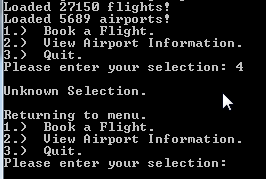
\includegraphics{Validation1.png}

\textit{The screenshot above shows that the main menu checks to determine if a valid choice form the menu is entered.}

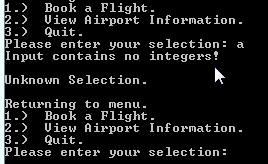
\includegraphics{Validation2.png}

\textit{The screenshot above shows that the main menu checks that an integer is entered as your selection.}

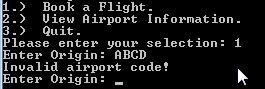
\includegraphics{Validation3.png}

\textit{The screenshot above shows that the origin airport code selection checks whether the airport code exists in the loaded data and that the check works for alphabetic inputs.}

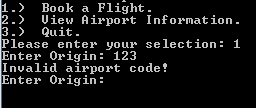
\includegraphics{Validation4.png}

\textit{The screenshot above shows that the origin airport code selection checks whether the airport code exists in the loaded data and that the check works for numeric inputs.}

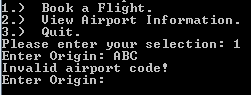
\includegraphics{Validation5.png}

\textit{The screenshot above shows that the origin airport code selection will show that the code is invalid even if it is completely alphabetic and 3 characters long in the case that the airport code doesn't exist in the loaded data.}

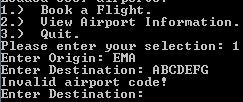
\includegraphics{Validation7.png}

\textit{The screenshot above shows that the destination airport code selection also checks and validates input. I decided not to show all different kinds of data in this input as it runs all of the same checks as the origin airport code selection.}

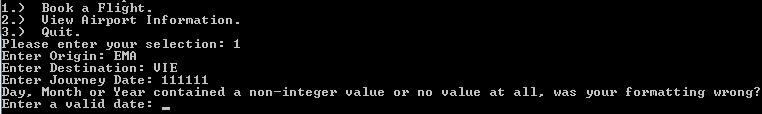
\includegraphics[scale=0.9]{Validation8.png}

\textit{The screenshot above shows that a date that doesn't follow the format DD/MM/YYYY won't be accepted and that the user will be informed of this.}

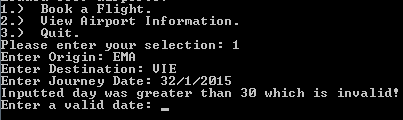
\includegraphics{Validation9.png}

\textit{The screenshot above shows that when a day that is greater than 30 is inputted, the program won't accept the input and will ask the user to enter a valid date.}

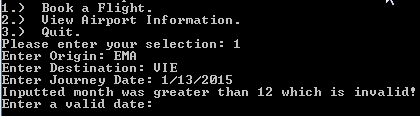
\includegraphics{Validation10.png}

\textit{The screenshot above shows that when a month that is greater than 12 is inputted, the program won't accept the input and will ask the user to enter a valid date.}

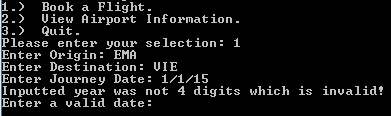
\includegraphics{Validation11.png}

\textit{The screenshot above shows that when a year that isn't 4 characters long is inputted, the program won't accept the input and will ask the user to enter a valid date.}

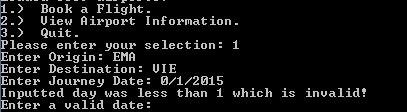
\includegraphics{Validation12.png}

\textit{The screenshot above shows that when a day that is less than 0 is entered, the program won't accept the input and will ask for a valid date to be entered.}

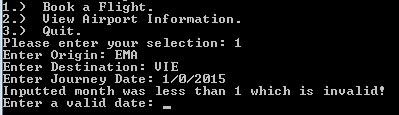
\includegraphics{Validation13.png}

\textit{The screenshot above shows that when a month that is less than 0 is entered, the program won't accept the input and will ask for a valid date to be entered}

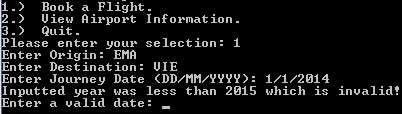
\includegraphics{Validation14.png}

\textit{The screenshot above shows that when a year that is less than 2014 is entered, the program won't accept the input and will ask for a valid date to be entered}

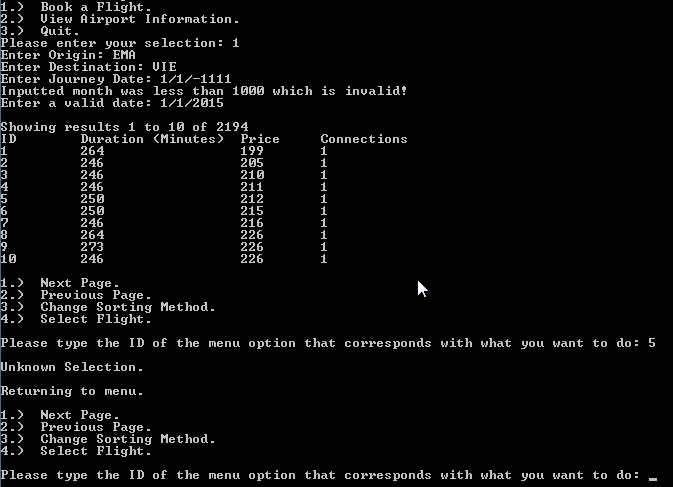
\includegraphics{Validation15.png}

\textit{The screenshot above shows that when an invalid menu option is selected in the trip display screen, the program will re-display the menu and ask for the input again.}

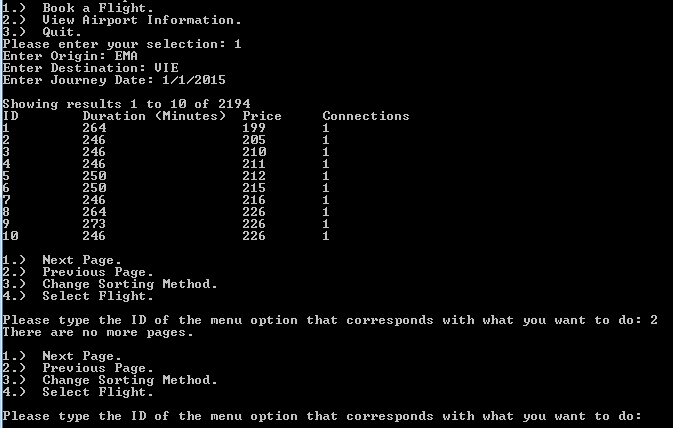
\includegraphics{Validation16.png}

\textit{The screenshot above shows that when you select to go to a previous page, but you are already at the first page, it will tell you that there are no more pages.}

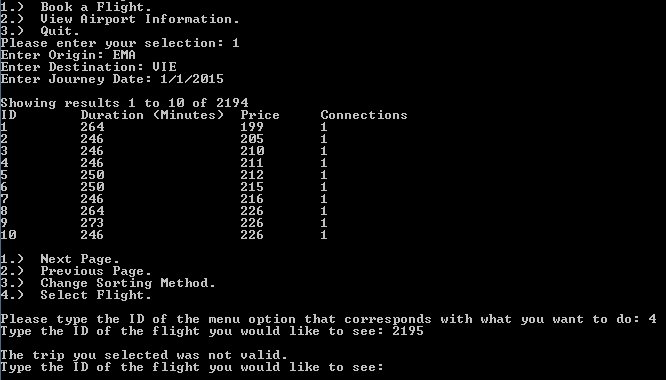
\includegraphics{Validation17.png}

\textit{The screenshot above shows that when you enter the ID of a trip that doesn't exist, the program won't accept the input and will alert the user to their mistake and request a different input.}

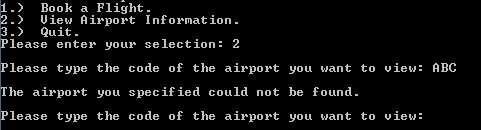
\includegraphics{Validation18.png}

\textit{The screenshot above shows that you can't input an airport code that doesn't exist in the data system as the program will ask you to input another airport code.}

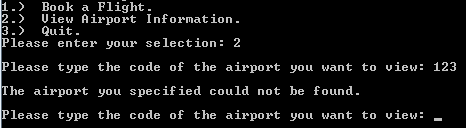
\includegraphics{Validation19.png}

\textit{The screenshot above shows that you can't input numeric characters for your airport code as they will be checked against the codes existing in the system and none will be found, therefore the program will ask for you to enter another airport code.}

\newpage

\subsection{Airports Data File Validation}
Below are screenshots of the validation checks being tested on the airports datafile when it is loaded into the program.

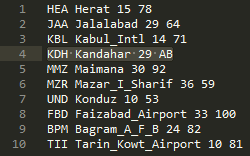
\includegraphics{Data1.png}

\textit{The screenshot above shows the data that will be used in the test below. There is an error in the file on line 4 where the connection time isn't an integer but is instead the characters AB.}

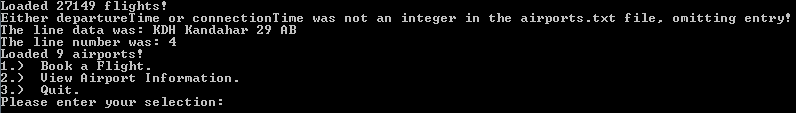
\includegraphics[scale=0.85]{DataValidation1.png}

\textit{The screenshot above shows that the program detected the error in the file and skipped over that line of data but loaded all of the other data in the file. The error in the data was reported so it could be found by the user.}

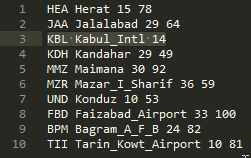
\includegraphics{Data2.png}

\textit{The screenshot above shows the data that will be used in the test below. There is an error in the file on line 3 where the connection time is missing from the data.}

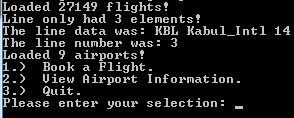
\includegraphics{DataValidation2.png}

\textit{The screenshot above shows that the program detected the error in the file and skipped over that line of data but loaded all of the other data in the file. The error in the data was reported so it could be found by the user.}

\newpage

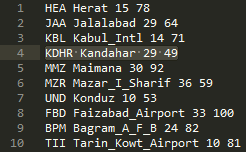
\includegraphics{Data3.png}

\textit{The screenshot above shows the data that will be used in the test below. There is an error in the file on line 4 where the airport code is 4 characters long rather than the three it is supposed to be.}

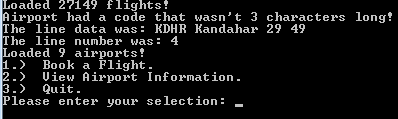
\includegraphics{DataValidation3.png}

\textit{The screenshot above shows that the program detected the error in the file and skipped over that line of data but loaded all of the other data in the file. The error in the data was reported so it could be found by the user.}

\newpage

\subsection{Flights Data File Validation}
Below are screenshots of the validation checks being tested on the flights datafile when it is loaded into the program.

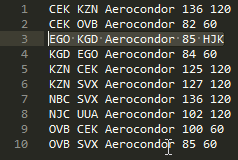
\includegraphics{Data4.png}

\textit{The screenshot above shows the data that will be used in the test below. There is an error in the file on line 4 where the flight duration isn't an integer but is instead the characters HJK.}

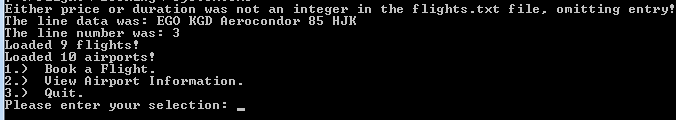
\includegraphics[scale=0.85]{DataValidation4.png}

\textit{The screenshot above shows that the program detected the error in the file and skipped over that line of data but loaded all of the other data in the file. The error in the data was reported so it could be found by the user.}

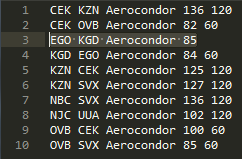
\includegraphics{Data5.png}

\textit{The screenshot above shows the data that will be used in the test below. There is an error in the file on line 3 where the flight duration is missing from the data.}

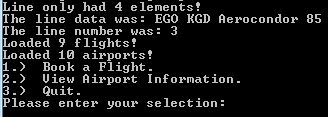
\includegraphics{DataValidation5.png}

\textit{The screenshot above shows that the program detected the error in the file and skipped over that line of data but loaded all of the other data in the file. The error in the data was reported so it could be found by the user.}

\newpage

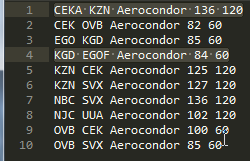
\includegraphics{Data6.png}

\textit{The screenshot above shows the data that will be used in the test below. There are two errors in this file, one on line 1 and one on line 4. The error on line 1 is with the origin airport code as it is 4 characters long rather than 3. The error on line 4 is with the destination airport code as it is 4 characters long rather than 3.}

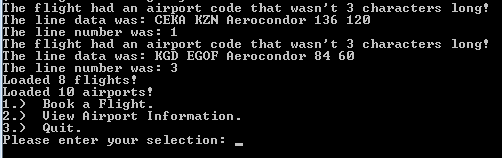
\includegraphics{DataValidation6.png}

\textit{The screenshot above shows that the program detected the two errors in the file and skipped over both lines of data but loaded all of the other data in the file. The error in the data was reported so it could be found by the user.}

\section{Functionality}
\begin{table}[h]
\begin{tabular}{|p{150pt} | p{60pt} | p{250pt}|}
\hline
\textbf{Functionality} & \textbf{Y(Complete) P(Partial) N(None)} & \textbf{Comments (e.g. more details on what is not working etc.)} \\ \hline
Data import (from files) & Y & Fully working as expected. \\ \hline
User input (from keyboard) & Y & Fully working as expected. \\ \hline
List flights for an airport & Y & Fully working as expected. \\ \hline
Search for direct flights & Y & Fully working as expected. \\ \hline
Search via 1 connection & Y & Fully working as expected. \\ \hline
Search via 2 connections & Y & Fully working as expected. \\ \hline
Sorting itineraries by cost/time & Y & Fully working as expected. \\ \hline
Book flight/"print" ticket & Y & File is saved to disk under a name specified by the user using keyboard input. Works as expected. \\ \hline
Handling dates correctly & Y & All dates are converted to the format specified in the specification. Works as expected. \\ \hline
Error handling & Y & Lots of validation is done on the data and all errors I can think of have been handled. \\ \hline
\end{tabular}
\end{table}
\end{document}